\section{问题二：玻璃类型判别与亚类划分}
\label{sec:problem2}

\subsection{建模口径与总体思路}
问题二关注的是已分类文物的成分规律，而不是对表单3未知文物作出最终归类；后者留在问题三处理。
因此，本文以表单2的67个有效采样点为分析单位，并将同一文物的多个采样点视为相关观测。
其中铅钡玻璃49点、高钾玻璃18点，来自56件文物。
为避免将同一文物的不同部位同时用于训练与验证，所有二分类性能均在按文物编号分组的5折验证中计算。

各成分已在数据预处理阶段闭合、近零替换并进行CLR变换，故本节不再重复处理零值或剔除异常值。
纹饰、颜色和整体风化状态不进入二分类器：玻璃类型本身是待解释标签，且这些辅助字段不能替代化学检测证据；本节只以14个CLR成分坐标建立可复核的化学判别规则。
模型链为“信息增益决策树给出规则---PLS--DA检验判别稳定性并排序变量重要性---分类型K-means进行亚类划分”。

\subsection{高钾与铅钡玻璃二分类}
\subsubsection{可解释决策规则}
设第$i$个采样点的CLR成分向量为$\bm z_i$，类别$T_i\in\{1,2\}$分别表示铅钡和高钾玻璃。
在节点样本集$D$上，连续变量$z_j$的候选阈值$t$按信息增益
\begin{equation}
    \operatorname{Gain}(D,z_j,t)=H(D)-\frac{|D_-|}{|D|}H(D_-)-\frac{|D_+|}{|D|}H(D_+)
\end{equation}
选择，其中$D_-=\{i:z_{ij}<t\}$、$D_+=D\setminus D_-$，且
\begin{equation}
    H(D)=-\sum_{g=1}^{2}p_g\log_2p_g.
\end{equation}
该准则直接对应于“尽量使分裂后节点类别更纯”的考古判别需求；相较于深层黑箱模型，浅层树还能给出可审计的阈值规则\cite{breiman1984}。

在全部67点上拟合并以分组验证选择剪枝参数后，最终树仅含一个分裂节点：
\begin{equation}
    \mathrm{clr}(\mathrm{PbO})<1.7497\ \Rightarrow\ \text{高钾玻璃},\qquad
    \mathrm{clr}(\mathrm{PbO})\geq1.7497\ \Rightarrow\ \text{铅钡玻璃}.
    \label{eq:p2-tree-rule}
\end{equation}
这里的阈值比较的是PbO相对于该点全部成分几何均值的对数比，并非PbO原始百分数阈值。
这与铅矿助熔使铅钡玻璃PbO相对丰度更高的工艺机理相符。
不过，树在训练集上的完全分离不能视作泛化性能；按文物分组的平衡准确率为0.8333，说明少数文物的点位仍会跨过该单变量边界。

\begin{figure}[H]
    \centering
    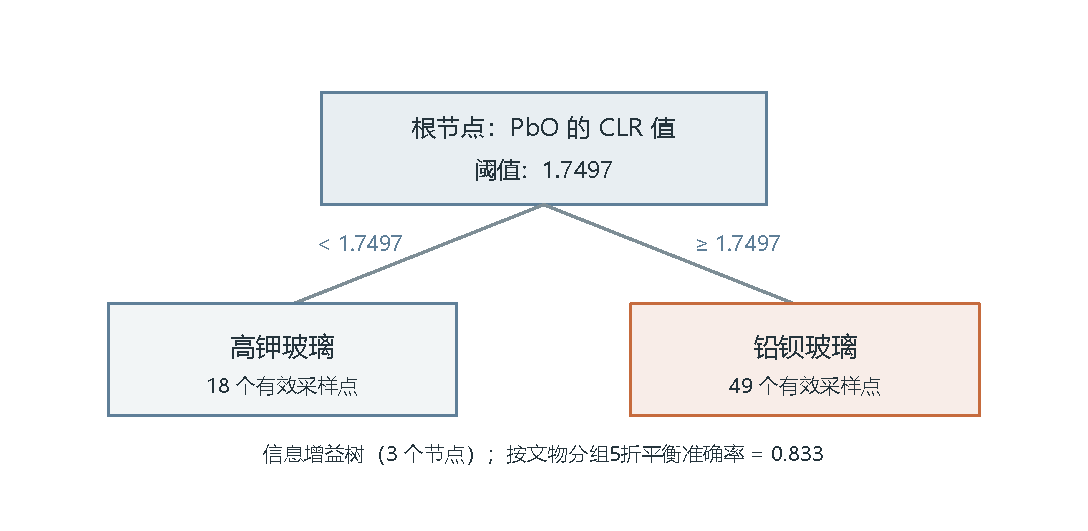
\includegraphics[width=0.82\textwidth]{figures/problem2_decision_tree.pdf}
    \caption{基于PbO的CLR可解释决策树}
    \label{fig:p2-decision-tree}
\end{figure}

\subsubsection{PLS--DA复核与重要成分}
为利用多成分的联合信息，将类别编码为两列哑变量矩阵$\bm Y$，并在训练折内对CLR坐标重新标准化。
偏最小二乘判别分析写为
\begin{equation}
    \bm X=\bm T\bm P^{\mathsf T}+\bm E_X,qquad
    \bm Y=\bm T\bm Q^{\mathsf T}+\bm E_Y,
    \label{eq:p2-plsda}
\end{equation}
其中潜变量$\bm T$同时解释成分矩阵$\bm X$和类别矩阵$\bm Y$。
在候选的1--5个潜变量中，1个潜变量取得最高的分组验证性能，故不继续增加自由度。
变量$j$的重要性按
\begin{equation}
    \operatorname{VIP}_{j}=\sqrt{14\cdot
    \frac{\sum_{a}\operatorname{SSY}_{a}w_{ja}^{2}}
    {\sum_{a}\operatorname{SSY}_{a}}}
    \label{eq:p2-vip}
\end{equation}
计算；其中$w_{ja}$为第$a$个潜变量的标准化权重，$\operatorname{SSY}_a$为该潜变量解释的类别平方和\cite{wold2001}。

\begin{table}[H]
    \centering
    \caption{两类玻璃判别的按文物分组验证结果}
    \label{tab:p2-binary-validation}
    \small
    \begin{tabular}{lccc}
        \toprule
        方法 & 潜变量数/树节点数 & 准确率 & 平衡准确率 / 宏平均F1 \\
        \midrule
        信息增益决策树 & 3个节点 & 0.9104 & 0.8333 / 0.8712 \\
        PLS--DA & 1个潜变量 & 0.9851 & 0.9722 / 0.9807 \\
        \bottomrule
    \end{tabular}
\end{table}

表\ref{tab:p2-binary-validation}表明，单一PbO相对丰度已经提供了直观的初筛规则，而一维PLS--DA利用其他成分后对不同文物的迁移更稳定。
因此，式\eqref{eq:p2-tree-rule}用于解释分类机理，PLS--DA作为后续未知样品判别的主要化学评分器；PLS--DA的输出是判别得分，不能误称为已校准概率。

\begin{figure}[H]
    \centering
    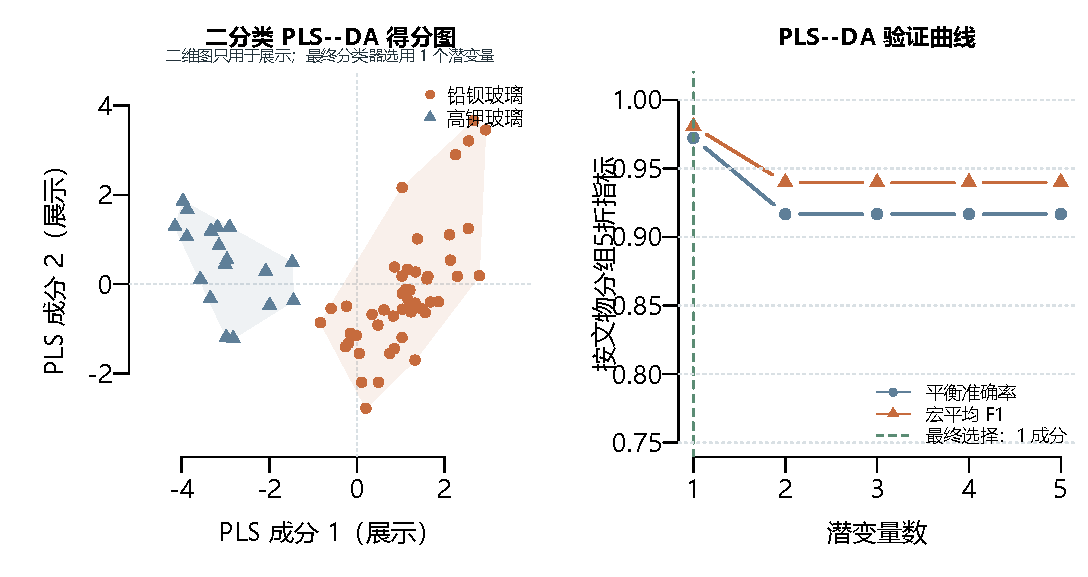
\includegraphics[width=\textwidth]{figures/problem2_binary_plsda.pdf}
    \caption{二分类PLS--DA二维展示与按文物分组验证曲线}
    \label{fig:p2-binary-plsda}
\end{figure}

\begin{table}[H]
    \centering
    \caption{二分类中VIP大于1的化学成分}
    \label{tab:p2-binary-vip}
    \small
    \begin{tabular}{ccccccc}
        \toprule
        排名 & 1 & 2 & 3 & 4 & 5 & 6 \\
        \midrule
        成分 & PbO & BaO & K$_2$O & SiO$_2$ & SrO & Al$_2$O$_3$ \\
        VIP & 1.915 & 1.566 & 1.505 & 1.193 & 1.109 & 1.100 \\
        \bottomrule
    \end{tabular}
\end{table}

PbO、BaO和K$_2$O分别对应铅钡助熔和草木灰助熔的主要差异，位居前三具有明确工艺解释；SiO$_2$、SrO和Al$_2$O$_3$补充刻画了基质与伴生矿物差异。
其余8种成分的VIP均不大于1，故不将它们作为两类玻璃的主要判别证据。

\subsection{分类型的亚类划分}
\subsubsection{特征与聚类数选择}
若直接在全部14个CLR坐标上聚类，低变异坐标会放大测量噪声且CLR坐标存在一条线性约束。
因此，对每个大类分别按组内CLR中位数绝对偏差（MAD）排序，保留变异最大的5个坐标，再在其组内标准化空间中求解K-means目标函数
\begin{equation}
    J_K=\sum_{g=1}^{K}\sum_{i\in C_g}\lVert\bm u_i-\bm\mu_g\rVert_2^2,
    \label{eq:p2-kmeans}
\end{equation}
其中$\bm u_i$为选定CLR坐标的标准化向量。
K-means以固定随机种子和100次随机起点运行；类别编号仅是按第一入模坐标中心排序的记号，不赋予年代或产地含义\cite{macqueen1967}。

聚类数不能只凭肘部图决定，本文同时要求每个最终簇至少含3个点，并检查平均轮廓系数、初始化稳定性和特征替换敏感性。
结果如表\ref{tab:p2-cluster-choice}：高钾组在$K=4$时的轮廓系数为0.660，且$K=5$开始出现单点簇；铅钡组从$K=4$到$K=5$的轮廓系数由0.292升至0.327，5簇的最小规模仍为8，故保留$K=5$。

\begin{table}[H]
    \centering
    \caption{两类玻璃的亚类划分设置与结果}
    \label{tab:p2-cluster-choice}
    \small
    \begin{tabularx}{\textwidth}{lXcS[table-format=3.3]S[table-format=1.3]c}
        \toprule
        玻璃类型 & 入模CLR成分（按组内MAD前五） & $K$ & {组内平方和} & {平均轮廓系数} & 簇规模 \\
        \midrule
        高钾 & PbO、BaO、Na$_2$O、SiO$_2$、SO$_2$ & 4 & 11.274 & 0.660 & 3, 8, 3, 4 \\
        铅钡 & Fe$_2$O$_3$、P$_2$O$_5$、K$_2$O、MgO、CuO & 5 & 91.937 & 0.327 & 11, 10, 11, 8, 9 \\
        \bottomrule
    \end{tabularx}
\end{table}

表\ref{tab:p2-cluster-choice}中的特征集合是各大类内部差异最大的成分，并不等价于表\ref{tab:p2-binary-vip}中区分两大类的成分。
图\ref{fig:p2-k-selection}同时呈现肘部下降和轮廓诊断：轮廓系数只作为检验分离度的辅助证据，不替代最小簇规模与稳定性约束。

\begin{figure}[H]
    \centering
    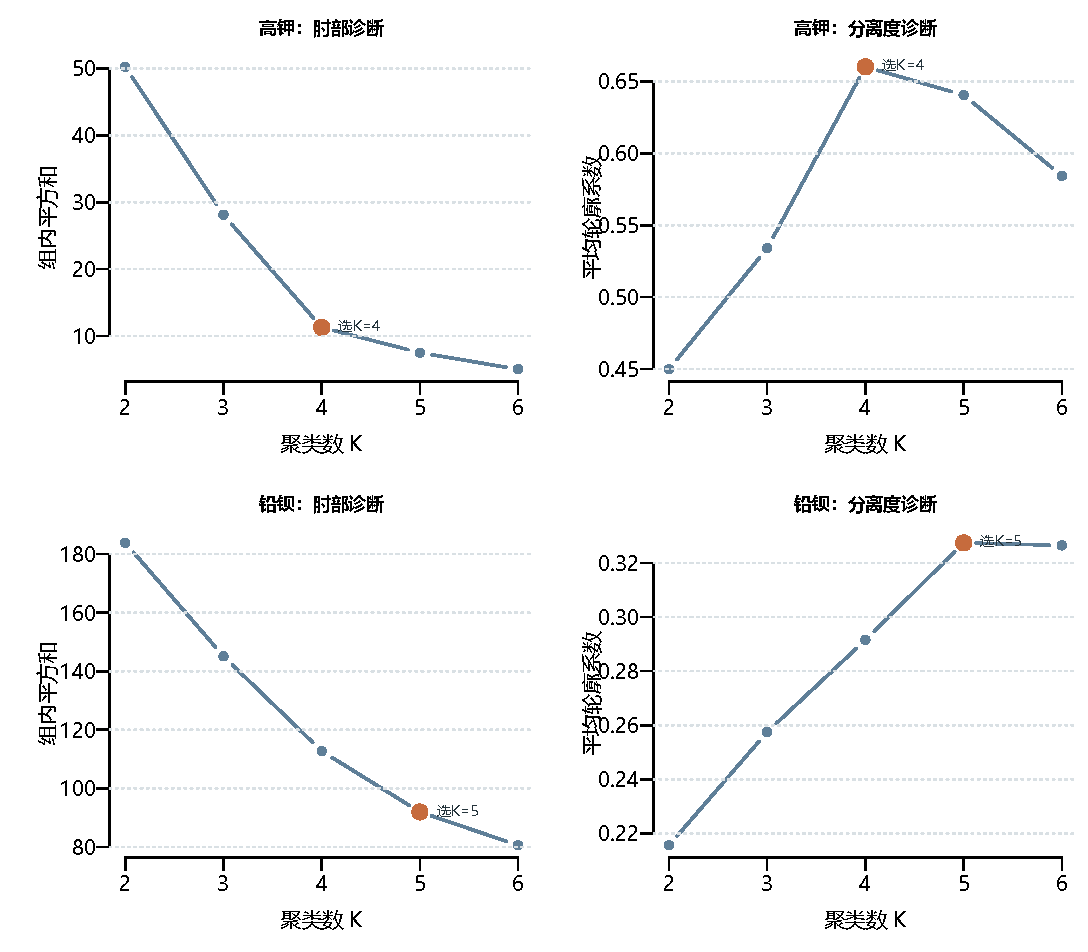
\includegraphics[width=0.90\textwidth]{figures/problem2_kmeans_selection.pdf}
    \caption{高钾与铅钡玻璃的K-means聚类数诊断}
    \label{fig:p2-k-selection}
\end{figure}

\begin{figure}[H]
    \centering
    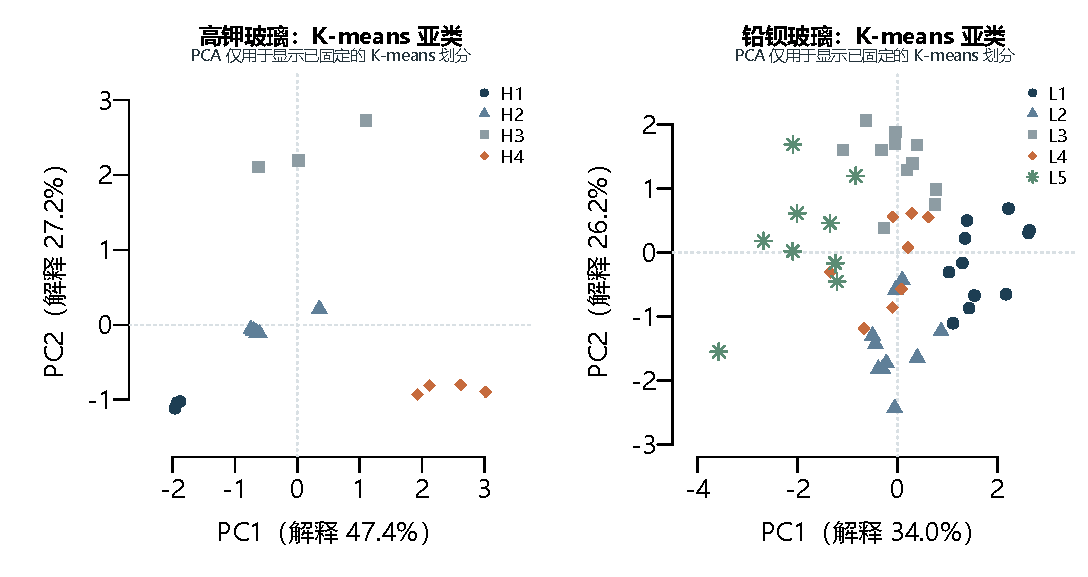
\includegraphics[width=\textwidth]{figures/problem2_kmeans_clusters.pdf}
    \caption{两类玻璃的K-means亚类在二维PCA投影中的显示}
    \label{fig:p2-kmeans-clusters}
\end{figure}

图\ref{fig:p2-kmeans-clusters}中的PCA仅将已确定的五维聚类空间投影到二维，坐标并未参与K-means的分配；因此二维重叠不改变表\ref{tab:p2-cluster-choice}中的高维聚类结论。
高钾玻璃的四个采样点亚类依次为：
\(\{01,04,05\}\)、
\(\{03\text{部位}1,07,09,10,12,18,22,27\}\)、
\(\{13,14,16\}\)和
\(\{03\text{部位}2,06\text{部位}1,06\text{部位}2,21\}\)。
铅钡玻璃五个亚类的完整采样点清单、全部14维中心及二次PLS--DA的VIP排序另存于支持材料，避免在正文中把长名单误排为文物级结论。

\subsubsection{亚类中心的成分特征}
聚类中心先在CLR空间取均值，再以逆CLR变换为和为$100\%$的组成；故表中的数值是近零替换口径下的几何中心，而不是各原始比例的算术平均。

\begin{table}[H]
    \centering
    \caption{高钾玻璃亚类的CLR逆变换中心（\%）}
    \label{tab:p2-high-centers}
    \small
    \begin{tabular}{ccccccc}
        \toprule
        亚类 & 样本数 & SiO$_2$ & K$_2$O & PbO & BaO & SO$_2$ \\
        \midrule
        H1 & 3 & 68.03 & 10.58 & 0.02 & 0.02 & 0.42 \\
        H2 & 8 & 95.26 & 0.57 & 0.03 & 0.02 & 0.02 \\
        H3 & 3 & 64.63 & 13.59 & 0.16 & 0.02 & 0.02 \\
        H4 & 4 & 74.29 & 2.17 & 0.63 & 1.86 & 0.02 \\
        \bottomrule
    \end{tabular}
\end{table}

H1与H3均表现为较高K$_2$O和较低SiO$_2$，但H3的Na$_2$O中心为$2.84\%$，高于H1的$0.02\%$；H2以高SiO$_2$为主；H4则具有相对较高的PbO和BaO。
这说明高钾玻璃内部并非单一配方，但小簇H1和H3各仅含3点，应理解为待进一步考古材料验证的组成型，而非确定的工艺谱系。

\begin{table}[H]
    \centering
    \caption{铅钡玻璃亚类的CLR逆变换中心（\%）}
    \label{tab:p2-lead-centers}
    \small
    \begin{tabular}{ccccccccc}
        \toprule
        亚类 & 样本数 & SiO$_2$ & MgO & Fe$_2$O$_3$ & CuO & PbO & BaO & P$_2$O$_5$ \\
        \midrule
        L1 & 11 & 26.94 & 0.03 & 0.02 & 3.62 & 40.68 & 22.78 & 1.65 \\
        L2 & 10 & 53.14 & 1.17 & 0.03 & 1.43 & 28.10 & 10.21 & 0.08 \\
        L3 & 11 & 32.60 & 1.00 & 0.56 & 1.34 & 46.29 & 2.64 & 8.87 \\
        L4 & 8 & 54.92 & 0.02 & 0.68 & 0.75 & 29.45 & 9.74 & 0.30 \\
        L5 & 9 & 46.73 & 0.93 & 1.28 & 0.12 & 35.90 & 3.90 & 1.36 \\
        \bottomrule
    \end{tabular}
\end{table}

铅钡亚类的差异主要体现在PbO--BaO组合以及Fe$_2$O$_3$、P$_2$O$_5$和CuO的伴生含量：L1具有较高PbO和BaO，L3的PbO和P$_2$O$_5$中心最高，而L5的Fe$_2$O$_3$中心最高、CuO中心最低。
与此一致，亚类PLS--DA的VIP前五项为MgO、CuO、Fe$_2$O$_3$、P$_2$O$_5$和K$_2$O；高钾亚类的VIP前五项为SiO$_2$、SO$_2$、Na$_2$O、BaO和SnO$_2$。
这些VIP仅描述已获得聚类标签后的分离方向，不能反过来证明聚类为唯一真值。

\begin{figure}[H]
    \centering
    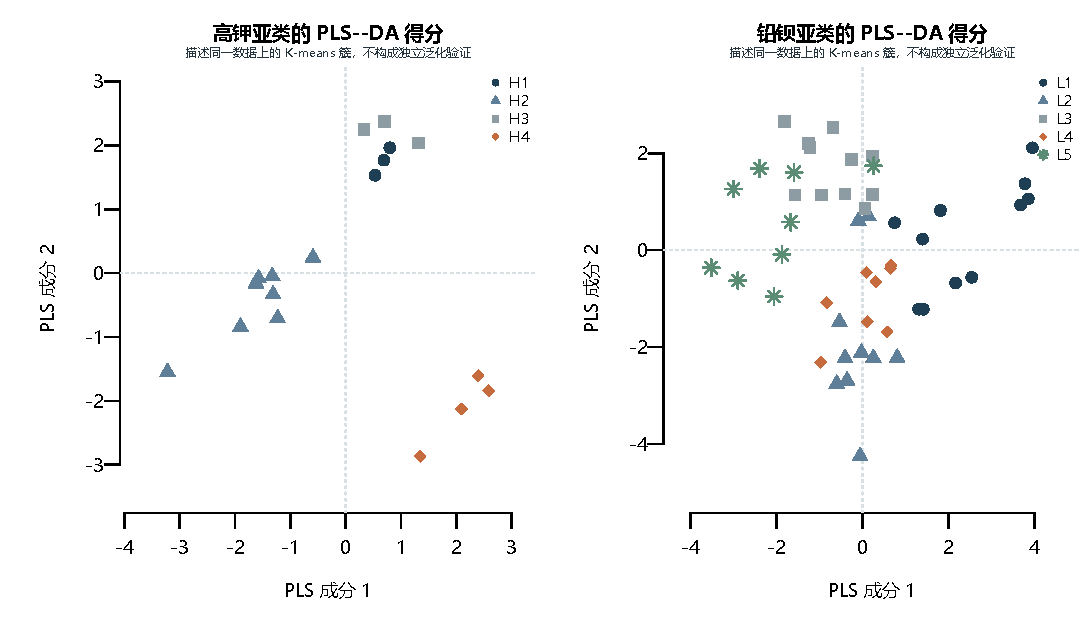
\includegraphics[width=\textwidth]{figures/problem2_subclass_plsda.pdf}
    \caption{两类玻璃亚类的PLS--DA描述性得分图}
    \label{fig:p2-subclass-plsda}
\end{figure}

图\ref{fig:p2-subclass-plsda}以K-means得到的同一批标签构造，故用于呈现各亚类在成分潜变量上的分离方向，不将图中的分离程度报告为独立测试集准确率。

\subsection{合理性与敏感性分析}
聚类结果的敏感性以调整兰德指数（ARI）衡量；ARI为1表示两次划分完全一致。
对高钾玻璃，标准化CLR坐标加入标准差0.03的独立噪声后，100次重算的ARI均为1；铅钡玻璃的平均ARI为0.998，最小值为0.944。
因此，已选成分的小幅测量扰动不会实质改变两类玻璃的亚类归属。

随机初始化则暴露出K-means的局部最优风险：100次单起点运行中，高钾和铅钡的平均ARI分别为0.874和0.889，最小值分别为0.537和0.421。
这正是最终计算固定种子并采用100次起点的原因，而不是将某一次随机运行当作结论。
特征筛选方面，高钾组将前五变量缩为前四或扩展为前六时ARI均为1；铅钡组对应ARI为0.668和0.893，说明其细分结构更依赖对Fe$_2$O$_3$、P$_2$O$_5$、K$_2$O、MgO和CuO的联合刻画。

\begin{figure}[H]
    \centering
    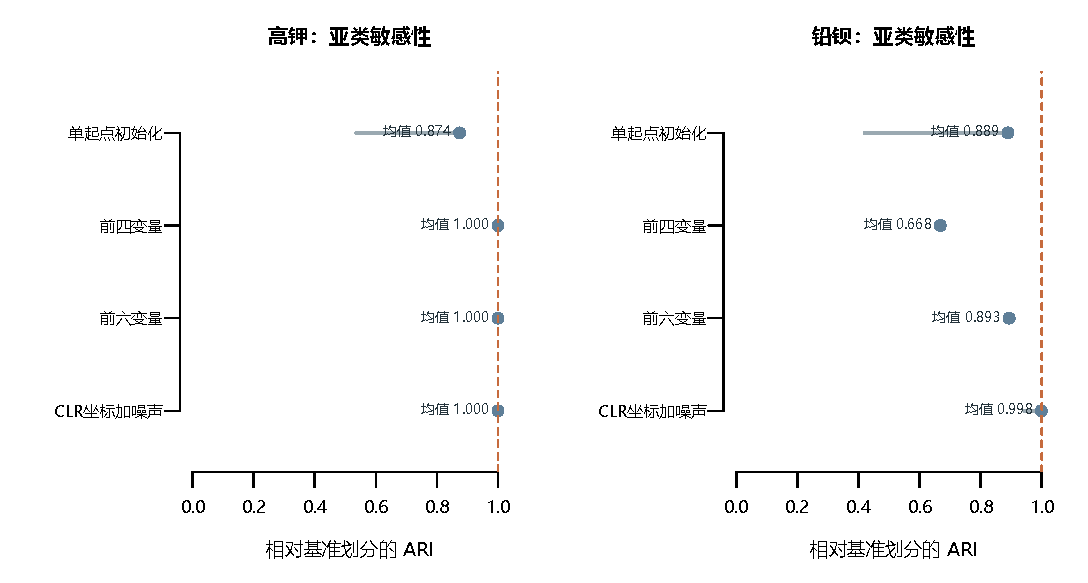
\includegraphics[width=\textwidth]{figures/problem2_kmeans_sensitivity.pdf}
    \caption{两类玻璃亚类的初始化、特征组合与小扰动敏感性}
    \label{fig:p2-kmeans-sensitivity}
\end{figure}

综上，二类玻璃的主判别规律稳健地指向PbO、BaO和K$_2$O等助熔相关成分；高钾的4个亚类对小扰动稳定但受样本量限制，铅钡的5个亚类具有中等轮廓分离度且对特征筛选更敏感。
亚类划分应作为后续样品比较与问题三敏感性分析的组成参照，而不应直接等同于独立的考古类型。
